% !TeX spellcheck = pt_BR
\documentclass[aspectratio=169, xcolor=dvipsnames]{beamer}
%Definições de tema
\setbeamertemplate{blocks}[rounded][shadow=false]
\usetheme{Madrid}
\setbeamertemplate{items}[square]
\setbeamertemplate{caption}[numbered]
\usecolortheme{beaver}
\setbeamercolor{frametitle}{bg=white!10!white}

\usefonttheme{professionalfonts}
\setbeamertemplate{itemize item}{\color[rgb]{0.8,0,0}$\blacksquare$}
\setbeamertemplate{itemize subitem}{\color[rgb]{0.8,0,0}$\blacksquare$}
\setbeamertemplate{itemize subsubitem}{\color[rgb]{0.8,0,0}$\blacksquare$}

%Definições de seção
\setcounter{secnumdepth}{3}
\setcounter{tocdepth}{2}

\usepackage{subfig}
\usepackage{xkeyval}
\usepackage{todonotes}
\presetkeys{todonotes}{inline}{}


\usepackage{helvet}
\renewcommand{\familydefault}{\sfdefault}
\usepackage{float}
\usepackage[brazil]{babel}
\usepackage[utf8]{inputenc}
\usepackage{graphicx, tikz}
\usepackage{url}
\usepackage{mathtools} % setas com texto
\usepackage{multicol}
\usepackage{listings}
\usepackage{lipsum}
\usepackage{scalefnt}
\usepackage{ragged2e}
\usepackage{etoolbox, verbatim}

% Listing
\lstset{
	numbers=left,
	stepnumber=1,
	numbersep=6pt,
	numberstyle=\small\color{black},
	basicstyle= \scriptsize,
%	keywordstyle=\color{black},
%	commentstyle=\color{black},
%	stringstyle=\color{black},
	tabsize=2
}
%Definições Listing - Linguagem Scala
\lstdefinelanguage{scala}{
morekeywords={abstract,case,catch,class,def,%
	do,else,extends,false,final,finally,%
	for,if,implicit,import,match,mixin,%
	new,null,object,override,package,%
	private,protected,requires,return,sealed,%
	super,this,throw,trait,true,try,%
	type,val,var,while,with,yield},
otherkeywords={=>,<-,<\%,<:,>:,\#,@},
sensitive=true,
morecomment=[l]{//},
morecomment=[n]{/*}{*/},
morestring=[b]",
morestring=[b]',
morestring=[b]"""
}

\let\olditem=\item%
\renewcommand{\item}{\olditem \justifying}

\title[Processamento Digital de Imagem]{\textbf{Processamento Digital de Imagem}\\\textit{Problema de Detecção Facial utilizando RCNN}}
\author[rodolfolabiapari@decom.ufop.br]{Rodolfo Labiapari Mansur Guimarães}
\institute[IFMG]{\begin{figure}
			\centering
			
\includegraphics[width=0.1\textwidth]{img/ufop.jpg}
		\end{figure}}
\institute[UFOP]{
	\textit{rodolfolabiapari@decom.ufop.br} \\
	Lattes: \url{http://goo.gl/MZv4Dc} \\
	Departamento de Computação -- Universidade Federal de Ouro Preto \\
	Ouro Preto - MG -- Brasil }

\date[\today]{Última Atualização: \today.}

\begin{document}


\frame{\titlepage}

\AtBeginSection[]
{
	\begin{frame}
	\frametitle{Sumário}
	\tableofcontents[]
	\end{frame}
}

\AtBeginSubsection[]
{
	\begin{frame}
	\frametitle{Sumário}
	\tableofcontents[
    currentsection,
    currentsubsection,
    hideothersubsections,
    %sectionstyle=show/hiden,
    subsectionstyle=show/shaded, ]
	\end{frame}
}

%\usebackgroundtemplate{
\includegraphics[trim=0cm 0cm 10cm 0cm, width=0.03\textwidth]{img/ufop.jpg}}

\section{Introdução}
	\subsection{Apresentação}
	\begin{frame}{Apresentação}
		\begin{itemize}
			\setlength\itemsep{2em}
			\item Pesquisas recentemente buscam focar em \textbf{detecção de face} em ambientes onde existe \cite{Garcia2004}
			\begin{itemize}
				\item \textbf{Maior complexidade};
				\item Sem perder sua \textbf{eficiência}.
			\end{itemize}

			\item As maiores dificuldades atuais são
			\begin{itemize}
				\setlength\itemsep{1.5em}
				\item Larga variações de visualização de faces humanas em fundos não-padronizados; e também
				\item A procura espacial onde cada face pode estar posicionada em diferentes posições e tamanhos  \cite{Haoxiang2015}.
			\end{itemize}
		\end{itemize}
	\end{frame}

	\subsection{Justificativa}
	\begin{frame}{Justificativa}
		\begin{itemize}
			\setlength\itemsep{2em}
			\item Sistemas computacionais \textbf{anteriores à redes neurais} possuíam características bastante \textbf{ineficientes} para imagens que tinham como propriedade fundos não-padronizados \cite{Garcia2004}.

			\item Sucesso de algoritmos que utilizam técnicas como a \textit{convolutional neural network} (CNN) \cite{LeCun1989} \\ \cite{LeCun1990H} \cite{LeCun1998G} \cite{Haoxiang2015}.
		\end{itemize}
	\end{frame}

\section{Referencial Teórico}
	\subsection{Rede Neural Convolucional}
		\begin{frame}[allowframebreaks]{Extração do Mapa de Características -}

			\begin{figure}[h]
				\centering
				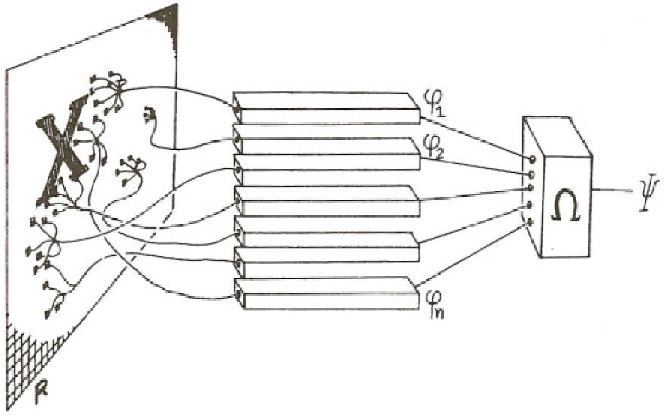
\includegraphics[width=0.56\linewidth]{img/single_layer_cnn.png}
				\caption{Visão geral do procedimento de detecção de objetos utilizando uma rede neural convolucional.}
				\label{fig:single_cnn.png}
			\end{figure}
		
			\begin{figure}[h]
				\centering
				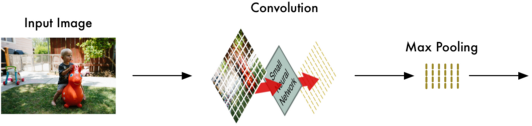
\includegraphics[width=1.0\linewidth]{img/features_map.png}
				\caption{Procedimento inicial da rede neural. Chamado Mapa de Características.}
				\label{fig:colored_cnn.png}
			\end{figure}
		
			\begin{itemize}
				\item \textbf{Subsampling} utiliza o algoritmo de \textit{max\_pooling}
				\begin{itemize}
					\item  Reduz o tamanho de amostras a ser processada \cite{Giusti2013}.
				\end{itemize}
			\end{itemize}
	
			\begin{figure}[H]
				\centering
				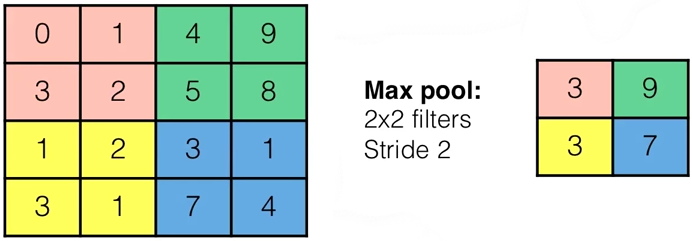
\includegraphics[width=0.7\linewidth]{img/max_pooling-2.png}
				\caption{O processo de seleção de melhores resultados. Procedimento executado pela função \texttt{max\_pooling} no \textit{subsampling} do mapa de características.}
				\label{fig:max_pooling.png}
			\end{figure}
		
		\end{frame}

		\begin{frame}[allowframebreaks]{Decisão Final usando Rede Neural Totalmente Conectada -}
			\begin{itemize}
				\setlength\itemsep{2em}
				\item As entradas da camada $ m $ são de um conjunto da camada anterior $ m-1 $ relacionados de uma forma contígua \cite{LeCun1998G}.
				
				\bigskip

					\begin{figure}[H]
						\centering
						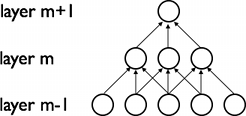
\includegraphics[width=0.6\linewidth]{img/layers_cnn.png}
						\caption{Exemplo das camadas de uma rede totalmente conectada em uma rede neural convolucional.}
						\label{fig:layers_cnn}
					\end{figure}
			\end{itemize}
		\end{frame}
	
		\begin{frame}{Visão Geral da Rede Neural Convolucional}
			\begin{figure}[h]
				\centering
				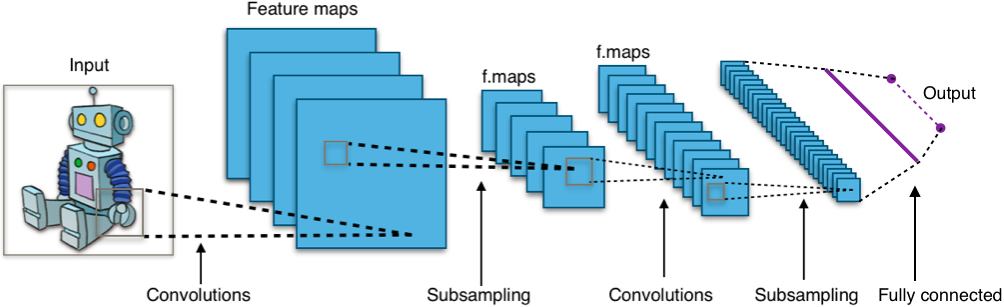
\includegraphics[width=1.0\linewidth]{img/visao_geral_convolucao.png}
				\caption{Arquitetura de reconhecimento de padrão \textit{convolutional neural network} final após todos os processos, utilizando dois mapas de características em sequência.}
				\label{fig:convolucao_teoria}
			\end{figure}
		\end{frame}


\section{Desenvolvimento} \label{sec:desenvolvimento}
	\subsection{Data Set}
		\begin{frame}{Data Set - Faces94}
			
			\begin{multicols*}{2}
				
				\begin{itemize}
					\item Disponível em \url{http://cswww.essex.ac.uk/mv/allfaces/faces94.html}.
					
					\bigskip
					
					\item Propriedades:
					\begin{itemize}
						\item Distância fixa da câmera;
						\item Solicitados para que falem enquanto as fotos foram tiradas;
						\item Imagens coloridas possuem plano de fundo verde;
						\item Variações naturais de rotação, movimento e posição
						\item Não possui variação de luminosidade.
					\end{itemize}
				
					\bigskip
					
					\item Total de 153 indivíduos, com imagens de resolução fixa no valor de $ 180 \times 200 $.
				\end{itemize}
				
				\begin{figure}[h]
					\centering
					\subfloat[Face 1]{{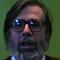
\includegraphics[width=0.25\linewidth]{img/94_colored.jpg} }}%
					\qquad
					\subfloat[Face 2]{{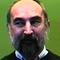
\includegraphics[width=0.25\linewidth]{img/94_colored_2.jpg} }}%
					
					\subfloat[Face 1 Cortada]{{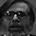
\includegraphics[width=0.25\linewidth]{img/94_cut.jpg} }}%
					\qquad
					\subfloat[Face 2 Cortada]{{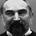
\includegraphics[width=0.25\linewidth]{img/94_cut_2.jpg} }}%
					\caption{As respectivas faces já processadas e prontas para treino.}%
					\label{fig:94_cut}%
				\end{figure}
				
			\end{multicols*}
		\end{frame}
	
		\begin{frame}{Data Set - FDDB}
			
			\begin{multicols*}{2}
				
				\begin{figure}[ht]
					\centering
					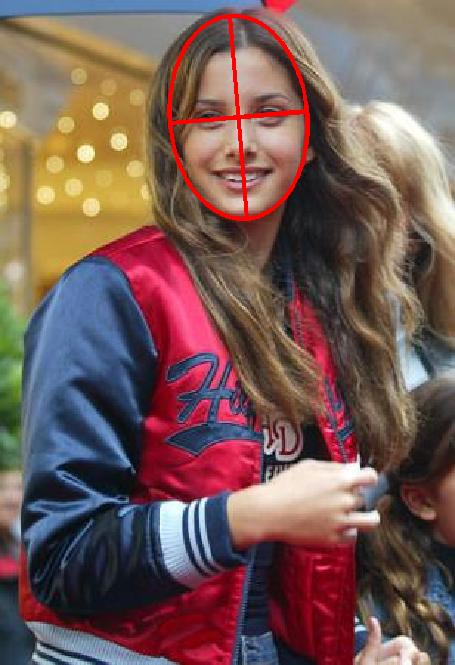
\includegraphics[width=0.5\linewidth]{img/data_set.jpg}
					\caption{Exemplo de identificação de rosto especificado pelo \textit{data set} disponibilizado pela Universidade de Massachusets Amherst.}
					\label{fig:mulher}
				\end{figure}
				
				\begin{figure}[h]
					\centering
					\subfloat[Não-face 1]{{
\includegraphics[width=0.25\linewidth]{img/fddb_cut.jpg} }}%
					\qquad
					\subfloat[Não-face 2]{{
\includegraphics[width=0.25\linewidth]{img/fddb_cut_2.jpg} }}%
					\qquad
					\subfloat[Não-face 3]{{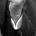
\includegraphics[width=0.25\linewidth]{img/fddb_cut_3.jpg} }}%
					\caption{Algumas imagens recortadas para treino de não-faces.}%
					\label{fig:fddb_cut}%
				\end{figure}
				
			\end{multicols*}
		\end{frame}
	
	\subsection{Treino, Teste e Validação}
		\begin{frame}{Treino, Teste e Validação}
			
			\begin{multicols*}{3}
				
				\textbf{Treino:}
				\begin{itemize}
					\setlength\itemsep{0.7em}
					\item FDDB-fold-\textbf{01}-ellipseList.txt
					\item FDDB-fold-\textbf{02}-ellipseList.txt
					\item FDDB-fold-\textbf{03}-ellipseList.txt
					\item FDDB-fold-\textbf{04}-ellipseList.txt
				\end{itemize}
				
				\bigskip
				
				\textbf{Teste:}
				\begin{itemize}
					\setlength\itemsep{0.7em}
					\item FDDB-fold-\textbf{05}-ellipseList.txt
					\item FDDB-fold-\textbf{06}-ellipseList.txt
					\item FDDB-fold-\textbf{07}-ellipseList.txt
					\item FDDB-fold-\textbf{08}-ellipseList.txt
				\end{itemize}
				
				\vspace{3cm}
				
				\textbf{Avaliação:}
				\begin{itemize}
					\setlength\itemsep{0.7em}
					\item FDDB-fold-\textbf{09}-ellipseList.txt
					\item FDDB-fold-\textbf{10}-ellipseList.txt
				\end{itemize}
			\end{multicols*}
		\end{frame}
	
	\subsection{Configurações da API neon}
		\begin{frame}{Configurações da API \textit{neon}}
			\begin{multicols*}{2}
				\begin{itemize}
					\item Camadas utilizadas na arquitetura da rede:
					\begin{itemize}
						\setlength\itemsep{0.7em}
						\item \textbf{\textit{Convolution}:} fshape=(5, 5, 4);
						\item \textbf{\textit{Pooling}:} fshape=(2, 2);
						\item \textbf{\textit{Convolution}:} fshape=(3, 3, 14);
						\item \textbf{\textit{Pooling}:} fshape=(2, 2);
						\item \textbf{\textit{Affine}:} nout=14;
						\item \textbf{\textit{Affine}:} nout=2.
					\end{itemize}
					
					\bigskip
					
					\item As configurações utilizadas para a realização dos testes foram:
					
					\begin{itemize}
						\setlength\itemsep{0.3em}
						\item \textbf{\textit{Batch size}:} 512;
						\item \textbf{\textit{Numbers of epoch}:} 1250;
						\item \textbf{\textit{Size of image} (altura e largura):} 36;
						\item \textbf{\textit{Learning Rate}:}; 0.01
						\item \textbf{\textit{Momentum}:} 0.9;
						\item \textbf{\textit{Format files}:} \texttt{.jpg};
						\item \textbf{\textit{Type of datas}:} inteiro não sinalizado de 8-bits.
					\end{itemize}
				\end{itemize}
		\end{multicols*}
		\end{frame}

		\begin{frame}{Configurações da API \textit{neon}}
			\begin{figure}[h]
				\centering
				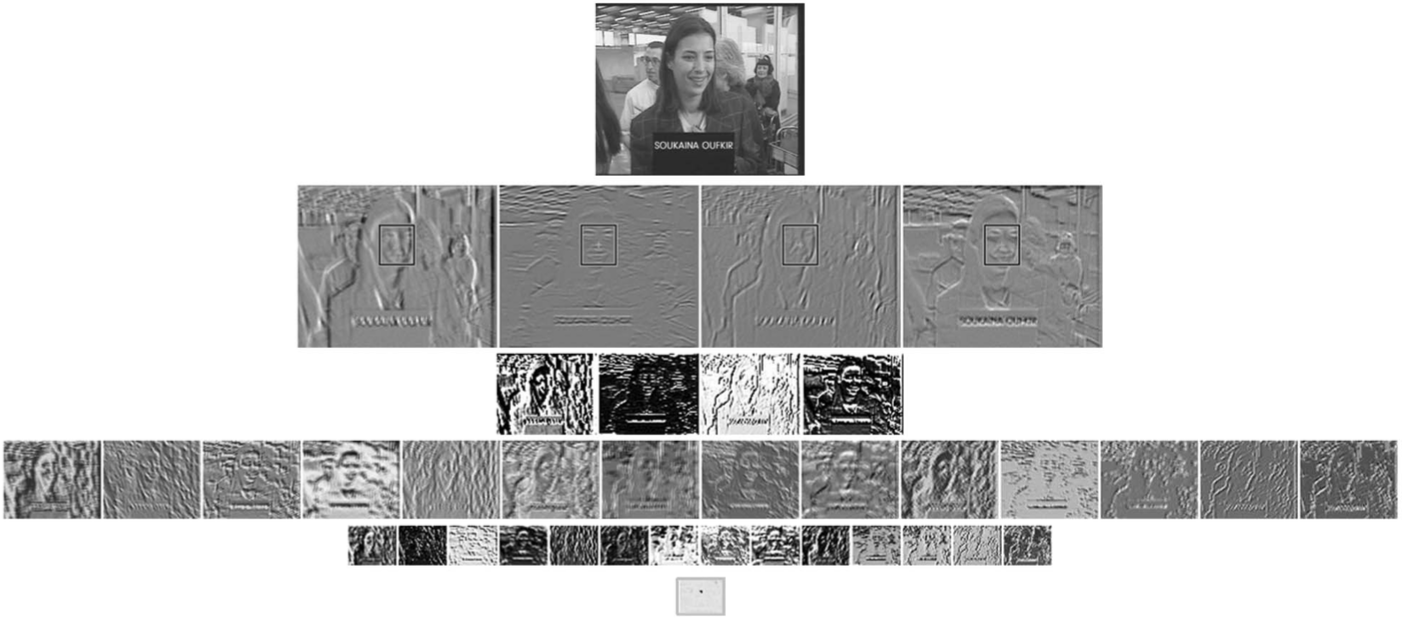
\includegraphics[width=1.0\linewidth]{img/archtecture.png}
				\caption{Exemplo prático do processo dos mapas de características \cite{Garcia2004}.}
				\label{fig:mapa}
			\end{figure}
		\end{frame}
	
\section{Experimentos}
	\begin{frame}{Experimentos}
		\begin{itemize}
			\setlength\itemsep{1em}
			\item Adaptou-se para o reconhecimento de regiões, também chamado de \textit{Region-based Convolutional Neural Network} (RCNN).
			
			\bigskip
			
			\item Foi feito um processamento de geração de regiões que:
			\begin{itemize}
				\setlength\itemsep{0.5em}
				\item Pega a imagem original a ser avaliada;
				\item Recorta-a em várias regiões de vários tamanhos diferentes;
				\item Redimensiona-as para o formato padrão de entrada da rede neural.
			\end{itemize}
		\end{itemize}
	\end{frame}

\section{Resultados}
	\begin{frame}{Resultados}
		\begin{table}[H]
			\centering
			\caption{Valores totais e percentuais de cada tipo de erro dos \textit{data sets} de validação.}
			\label{tab:erros}
			\begin{tabular}{|l|c|c||c|c|}
				\hline
				& \textbf{Numbers} & \textbf{\%}     & \textbf{Numbers} & \textbf{\%}     \\ \hline
				\textit{True Positives}  & 2995    & 55,391 & 2801    & 51,038 \\ \hline
				\textit{False Positives} & 2412    & 44,608 & 2687    & 48,961 \\ \hline \hline
				\textit{True Negatives}  & 239.142 & 49,694 & 239.347 & 54,662 \\ \hline
				\textit{False Negatives} & 242.078 & 50,305 & 198.515 & 45,337 \\ \hline \hline \hline
				\textbf{Total Regions}   & \textit{486.627} & \textit{100}    & \textit{443.350} & \textit{100}    \\ \hline
			\end{tabular}
		\end{table}
		\begin{itemize}
			\setlength\itemsep{1em}
			\item Total de 929.977 regiões.
			
			\item Cerca de $ 50\% $ de acerto em suas decisões.
		\end{itemize}
	\end{frame}
	\begin{frame}
		\begin{figure}[h]
			\centering
			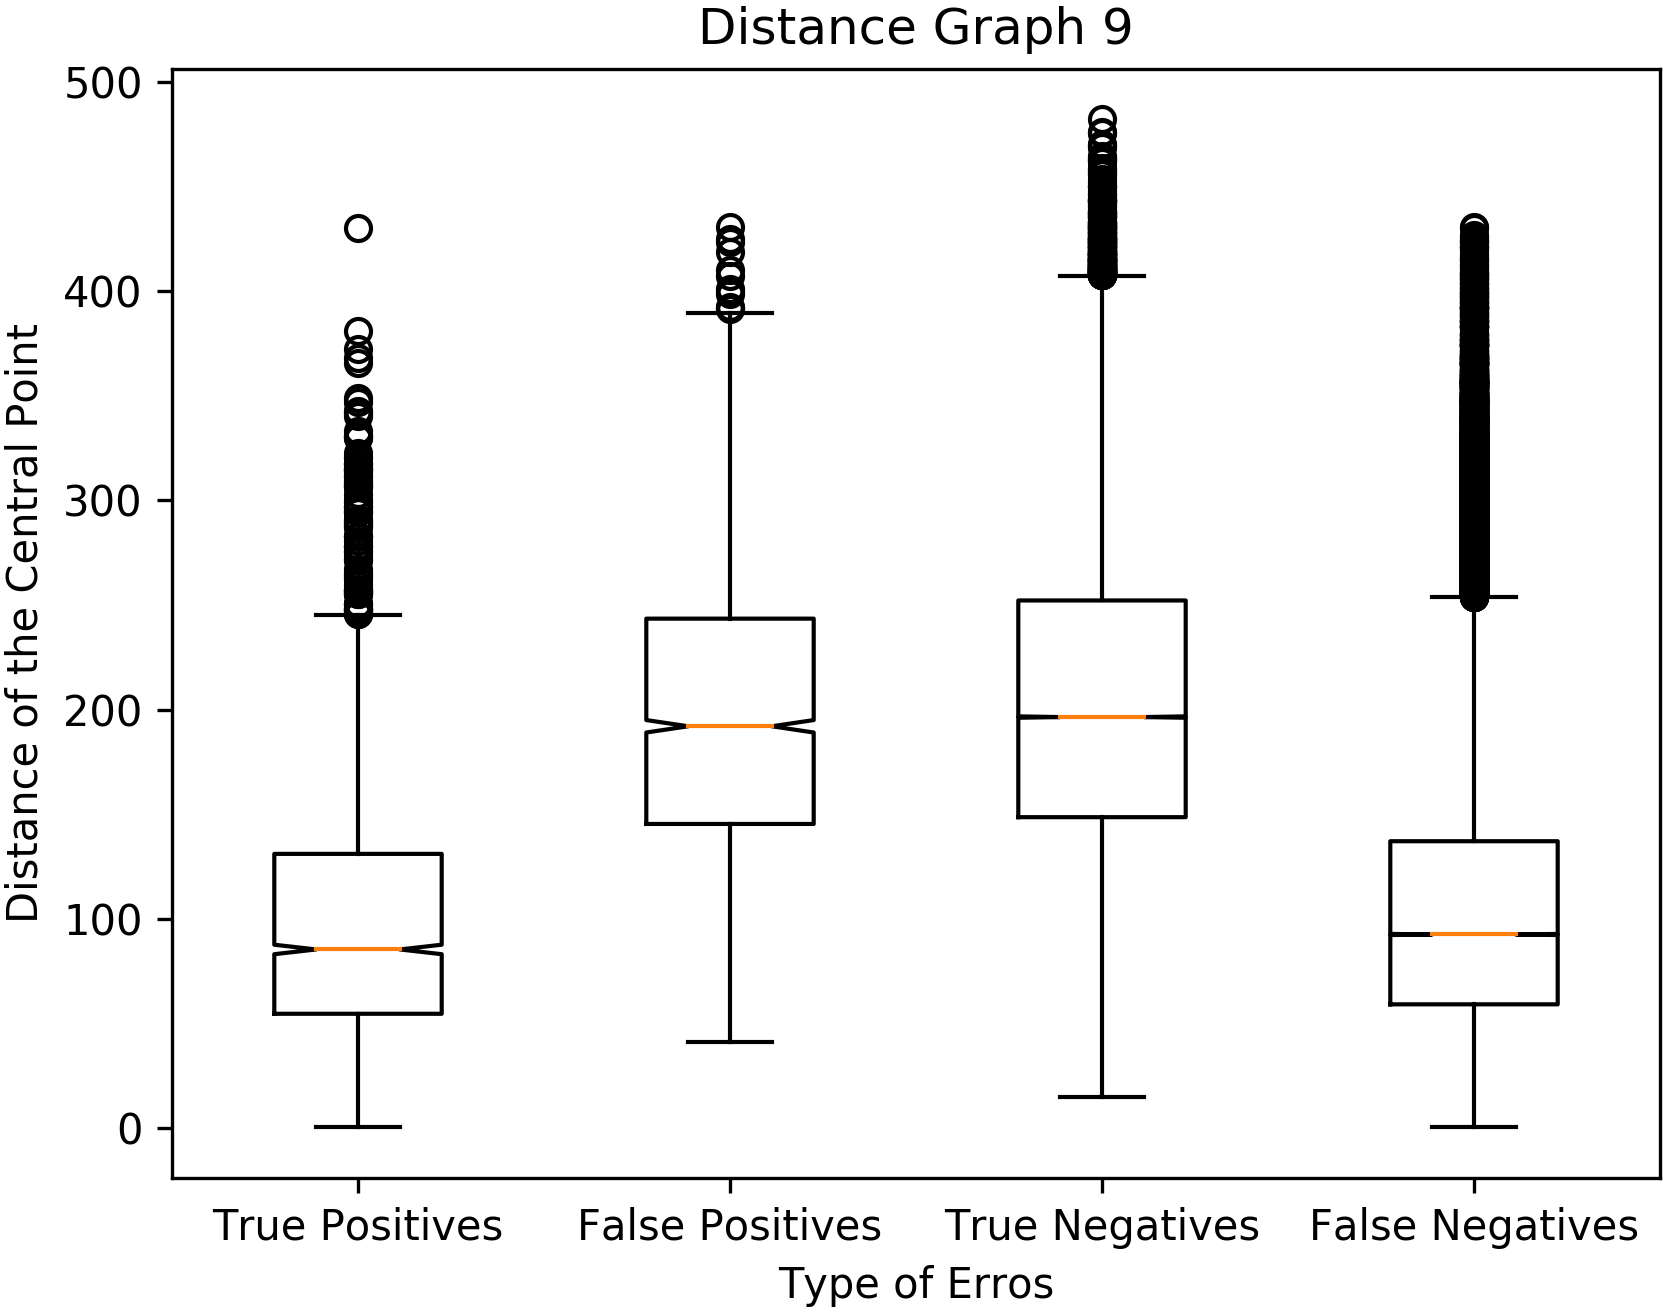
\includegraphics[width=0.7\linewidth]{img/boxplot-9.png}
			\label{fig:bp-9}
		\end{figure}
	\end{frame}
	\begin{frame}[plain]
		\begin{figure}[h]
			\centering
			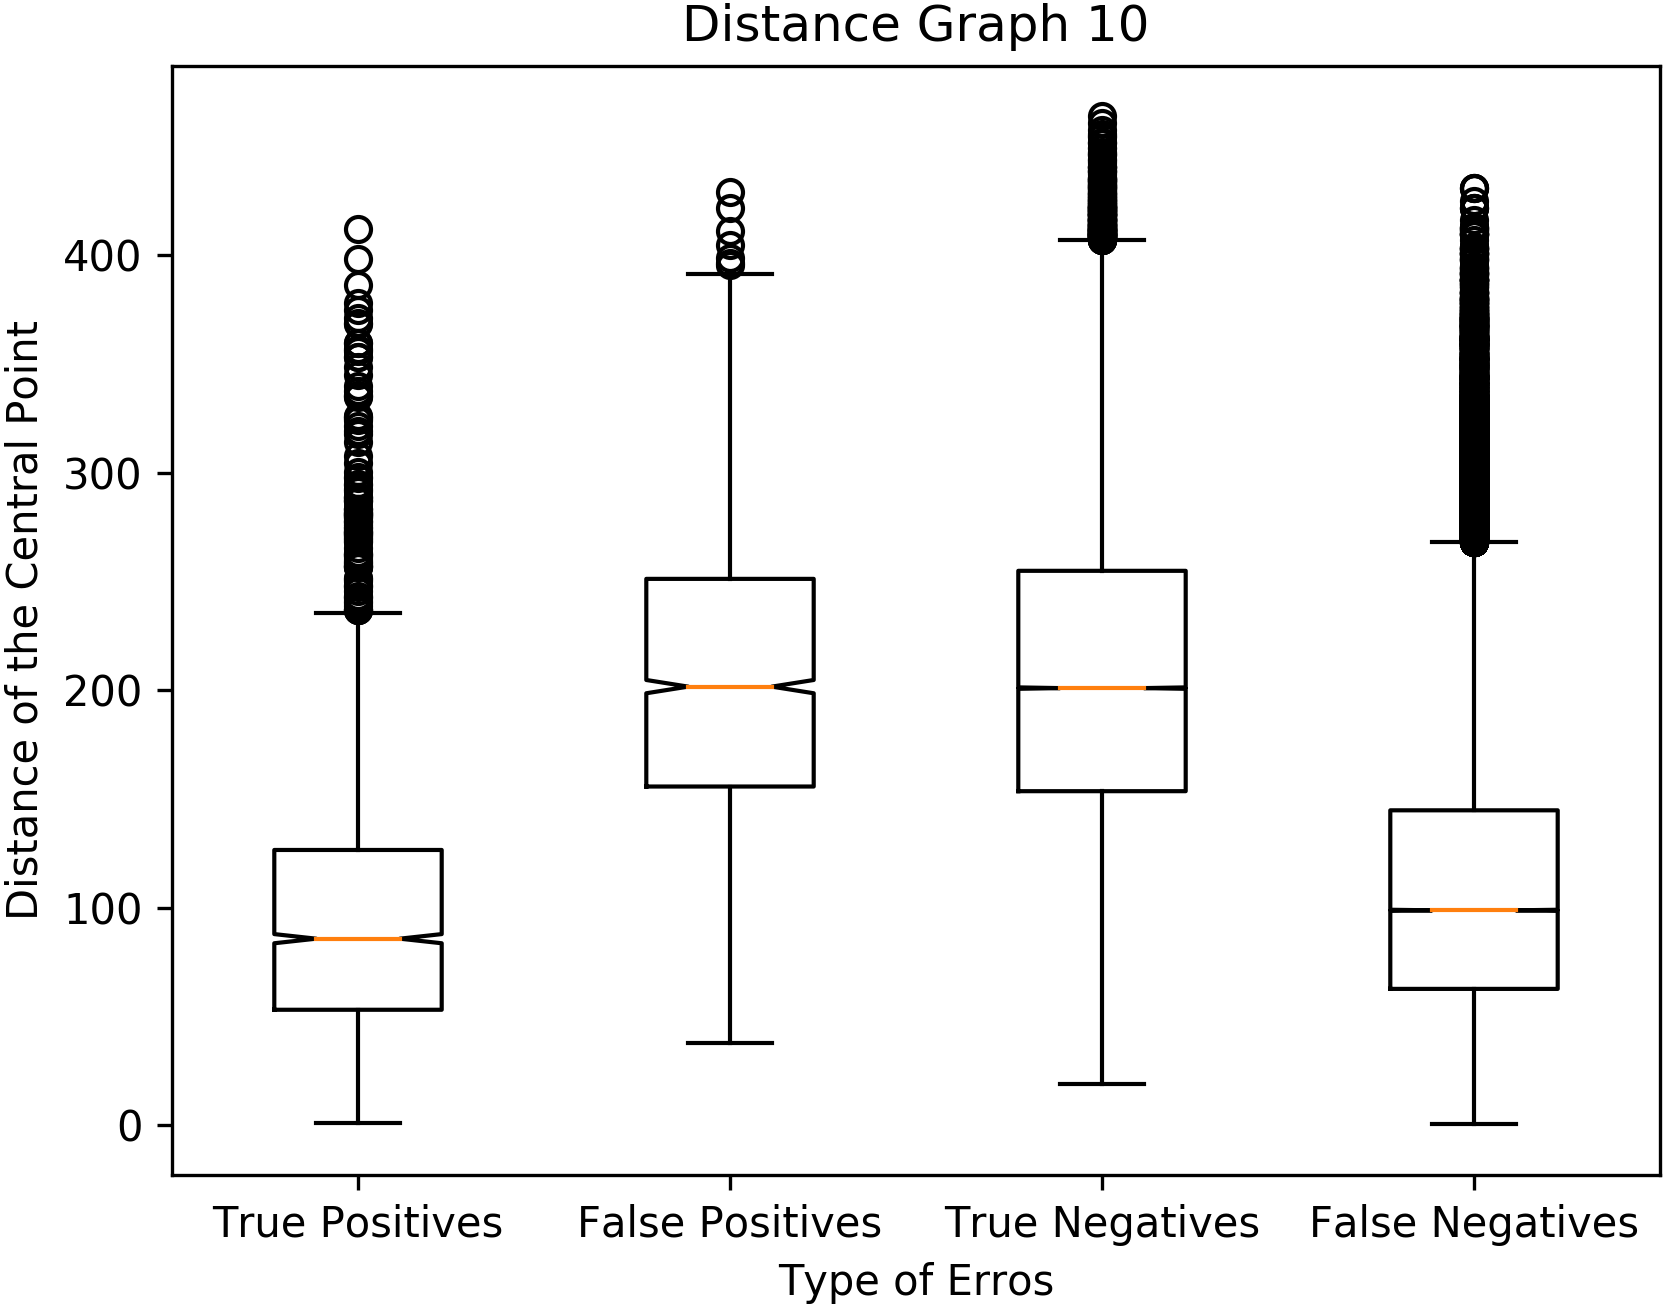
\includegraphics[width=0.72\linewidth]{img/boxplot-10.png}
			\label{fig:bp-10}
		\end{figure}
	\end{frame}
	
	\begin{frame}
		\begin{figure}[h]
			\centering
			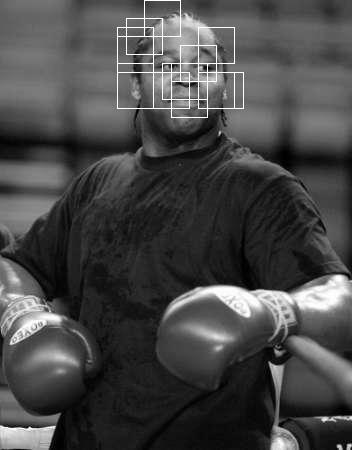
\includegraphics[width=0.9\linewidth]{img/detect.jpg}
			\caption{Exemplo de saída de uma foto após o processo de detecção.}
			\label{fig:detect_}
		\end{figure}
	\end{frame}

\section{Conclusão}
	\begin{frame}{Conclusão}
		\begin{itemize}
			\setlength\itemsep{1em}
			\item Conhecimento em teoria de inteligência artificial a configuração da rede e obtenção de resultados mais promissores.
			
			\item Conhecimento em teoria convolucional de imagens para adequar parâmetros para cada tipo de solução requisitada.
			
			\item Imagens e máscaras de pequeno porte dão resultados bons \cite{Garcia2004}.
		\end{itemize}
	\end{frame}

	\subsection{Trabalhos Futuros}
	\begin{frame}{Conclusão - Trabalhos Futuros}
		\begin{itemize}
			\setlength\itemsep{1em}
			
			\item Modificar o \textit{data set} de faces.
			
			\item Realizar um filtro nas imagens do \textit{data set FDDB}.
			
			\item Alterar o parâmetro de aprendizagem.
			
			\item Melhoria nas imagens de saída.
			
			\item Alterar a forma de saída da rede neural.
		\end{itemize}
	\end{frame}
\frame{\titlepage}

\bibliographystyle{sbc}
\bibliography{example}

\frame{\titlepage}

\section*{Anexos}
	\begin{frame}
		\begin{figure}[h]
			\centering
			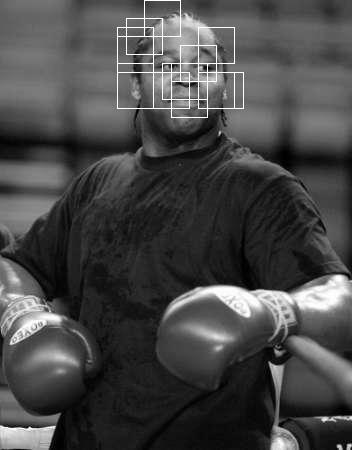
\includegraphics[width=0.9\linewidth]{img/detect.jpg}
			\caption{Exemplo de saída de uma foto após o processo de detecção.}
			\label{fig:detect_}
		\end{figure}
	\end{frame}
	
	\begin{frame}
		\begin{figure}[h]
			\centering
			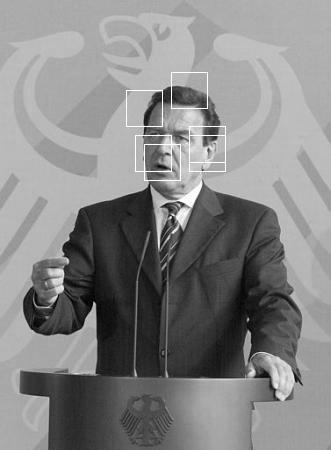
\includegraphics[width=0.6\linewidth]{img/detect_2.jpg}
			\caption{Resultado do processamento de reconhecimento de face no qual retornou com sucesso a face detectada.}
			\label{fig:detect_2}
		\end{figure}
	\end{frame}
	
	\begin{frame}
		\begin{figure}[h]
			\centering
			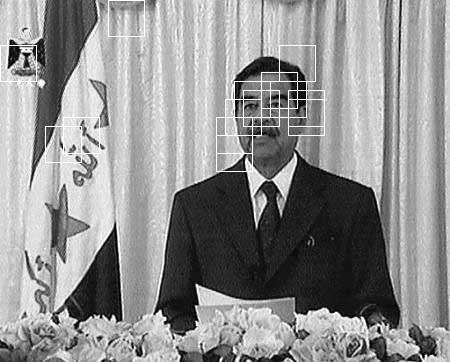
\includegraphics[width=0.57\linewidth]{img/detect_3.jpg}
			\caption{Exemplo de processamento de reconhecimento de face no qual não obteve sucesso total na detecção de todas as faces. Resultado com Falso Positivos, no emblema, na bandeira e na cortina.}
			\label{fig:detect_3}
		\end{figure}
	\end{frame}
	
	\begin{frame}
		\begin{figure}[h]
			\centering
			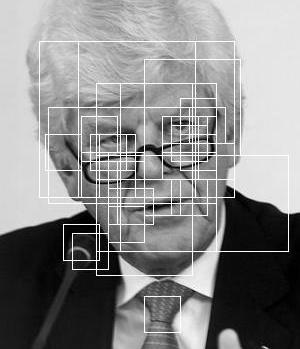
\includegraphics[width=0.4\linewidth]{img/detect_4.jpg}
			\caption{Processamento de reconhecimento de face no qual não obteve sucesso total na detecção de todas as faces. Resultado com Falso Positivos, na gravata, no terno e no microfone.}
			\label{fig:detect_4}
		\end{figure}
	\end{frame}
	
	\begin{frame}
		\begin{figure}[ht]
			\centering
			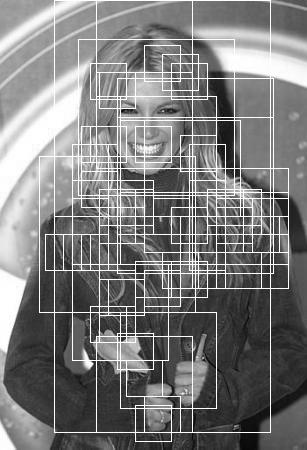
\includegraphics[width=0.4\linewidth]{img/detect_5.jpg}
			\caption{Exemplo de processamento de reconhecimento de face no qual não obteve sucesso total na detecção de todas as faces.}
			\label{fig:detect_5}
		\end{figure}
	\end{frame}


\end{document}
